\documentclass{cqupt}
%本模板由冯益青个人编写,基本符合毕业设计格式要求,但未获得重庆邮电大学教务处的授权
%使用如有不妥,概不负责
%修改后请使用XeLaTex编译,不要使用本文件中的图片和表格,查重会查到的~
%latex中下划线前要加上转义字符/
%进行个人信息设置
\title{xxxxxxxxxxxxx} %论文题目
\etitle{yyyyyyyyyyyyyyyy}
\author{冯益青} %作者姓名
\major{计算机科学与技术}	%专业
\date{\today} %日期,默认当日
\school{计算机科学与技术} %院系名称
\classnum{0491401} %班级
\stunum {2014211400} %学号
\instructor{xxx\hspace{2em}xxxx} %指导教师姓名和职称
\supervisor{} %答辩组负责人姓名
%填表时间以当前日期自动生成
\begin{document}
\maketitle
\makestatement
\pagenumbering{Roman} %摘要页码为大写罗马数字
\begin{cnabstract}{aa,bb,cc,dd,fff}

balabalabalabalablablablalblbalbalalblablalb

ballbalalblballblblalbalblalbalbllblballbablalbalblblalbalblalblbalballabllablblbalblabllbalbalbllba

		
\end{cnabstract}
%填写英文摘要内容和关键字
\begin{enabstract}{aaa,bbbb,cccc,ddd,fff}
With the rapid development of Internet, dddddddddddddddddddddddddddddddddddddd

fffffffffffffffffffffffffffffffffffffffffffffffffffffffffffffffffffff
ddddddddddddddddddddddddddddddddddddddddddddddddddddddddd
\end{enabstract}

\tableofcontents

\pagenumbering{arabic} %正文页码为阿拉伯数字
	
\clearpage
%正文内容从这里开始
\chapter{引言}
\section{研究背景和意义}
xxxxxxxxxxxxxxxxxxxxxxxxx

对xxxxxxxxxxxxxxxx的意义在于:

(1)yyyyyyyyyyyyyyyyyyyyy

(2)xxxxxxxxxxxxxxxxxxxx

(3)zzzzzzzzzzzzz

\section{国内外研究现状}
\subsection{国外研究现状}
xxxxxxxxxxxxxxxxxxxxxxxxxxxx
xxxxxxxxxxxxxxxxxxxxxxxxxxxxxxx
\subsection{国内研究现状}
yyyyyyyyyyyyyyyyyyyyyyyy
\section{主要内容和工作安排}
本文xxxxxxxxxxxxxxxxxxxxxxxxxxx。全文共分为6章,内容结构安排如下:

第1章为引言,ffffffffffffffffffff

第2章为yyyyyyyyyyyyyyyyyyyyyyyyyyyyy

第3章为qqqqqqqqqqqqqqqqqqqqqqqqqqqq

第4章为fffffffffffffffffffffffffffffffffffffffffffffffffff

第5章为yyyyyyyyyyyyyyyyyyyyyyyyyyyy

第6章qqqqqqqqqqqqqqqqqqqqqqqqqqqqq
\chapter{A}
\section{A1}
\subsection{A11}
XXXXXXXXXXXXXXXXXXXXXXXXXXXXXXXX
\subsection{A12}
FFFFFFFFFFFFFFFFFFFFFFFFFFFFFFFF
\begin{figure}[!htbp]
\centering
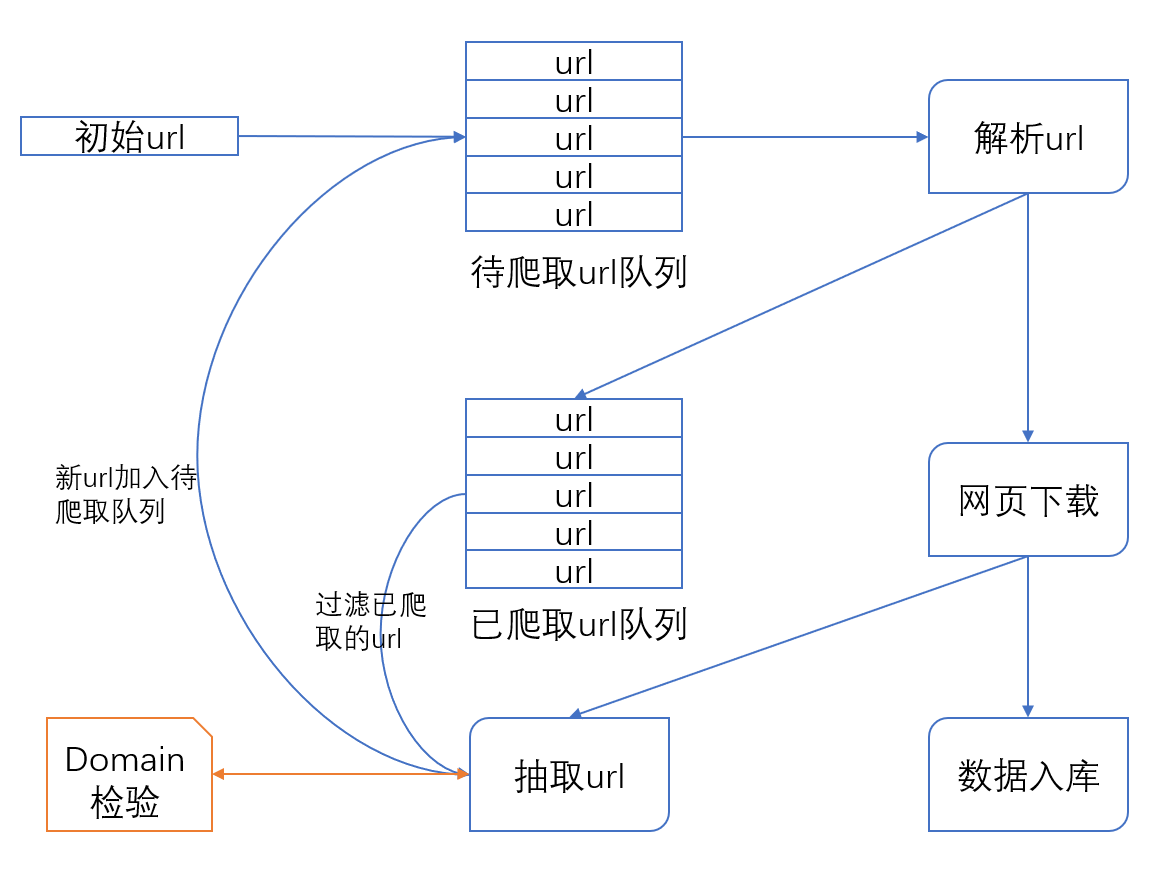
\includegraphics[height=7cm]{1.png}
\caption{网页爬取流程}\label{f1}
\end{figure}

\begin{table}[!htbp]
\caption{数据字段}\label{t1}
\centering
\begin{tabular}{llll}
\toprule
 字段名 & 类型 &字段名 &类型\\
\midrule
 title &varchar(200)&fav\_nums &int(11)\\
 create\_date & date &praise\_nums& int(11)\\
 url & varchar(300)&tags &varchar(200)\\
 url\_object\_id & varchar(50)&content & longmathrm\\
\bottomrule
\end{tabular}
\end{table}


\section{本章小结}
ZZZZZZZZZZZZZZZZZZZZZZZZZZ
%在每个新章节前将图片和表格计数器归零
\setcounter{figure}{0}
\setcounter{table}{0}
\chapter{B}
\section{B1}
QQQQQQQQQQQQQQQQQQQQQQQQQQQQQQQQQQQQQQQ

\begin{equation}
tf(t\mbox{ in }d) = \sqrt{\mathrm{frequency}}
\end{equation}


\begin{itemize}
\item 文档1。
\item 文档2
\item 文档3
\end{itemize}

%在每个新章节前将图片和表格计数器归零
\setcounter{figure}{0}
\setcounter{table}{0}

\chapter{总结与展望}
\section{主要工作总结}
FFFFFFFFFFFFFFFFFF
\section{后续研究展望}
YYYYYYYYYYYYYYYY

%参考文献
%假的bib参考文献。个人非常不喜欢LATEX自带的参考文献,于是自行手动添加参考文献
\begin{thebibliography}{99}
\addcontentsline{toc}{chapter}{参考文献}
\bibitem{1}
\bibitem{2}
\bibitem{3}

\end{thebibliography}

%致谢
\vspace*{-20pt}
\chapter*{致\hspace{1em}谢}
\addcontentsline{toc}{chapter}{致谢}
YYYYYYYYYYYYYYYYYYYYYYYYYYYYYYYYYYYYYYYYYYYYYYYYYYYYYYYYYYY

%附录
\clearpage
\appendix
\begin{appendices}
\chapter*{附\hspace{1em}录}

\end{appendices}

\end{document}